\chapter{Preprocessing Text}

Connect \widget{Word Cloud} to \widget{Corpus}. The visualization shows words, with their size corresponding to their frequency in the corpus. In this case, Word Cloud simply displays all the words and symbols found in the text. But this is often not what we want. We want to extract only meaningful units, such as semantically rich words. This is why we need text preprocessing.

\vspace{-0.2cm}
\begin{figure}[h]
  \centering
  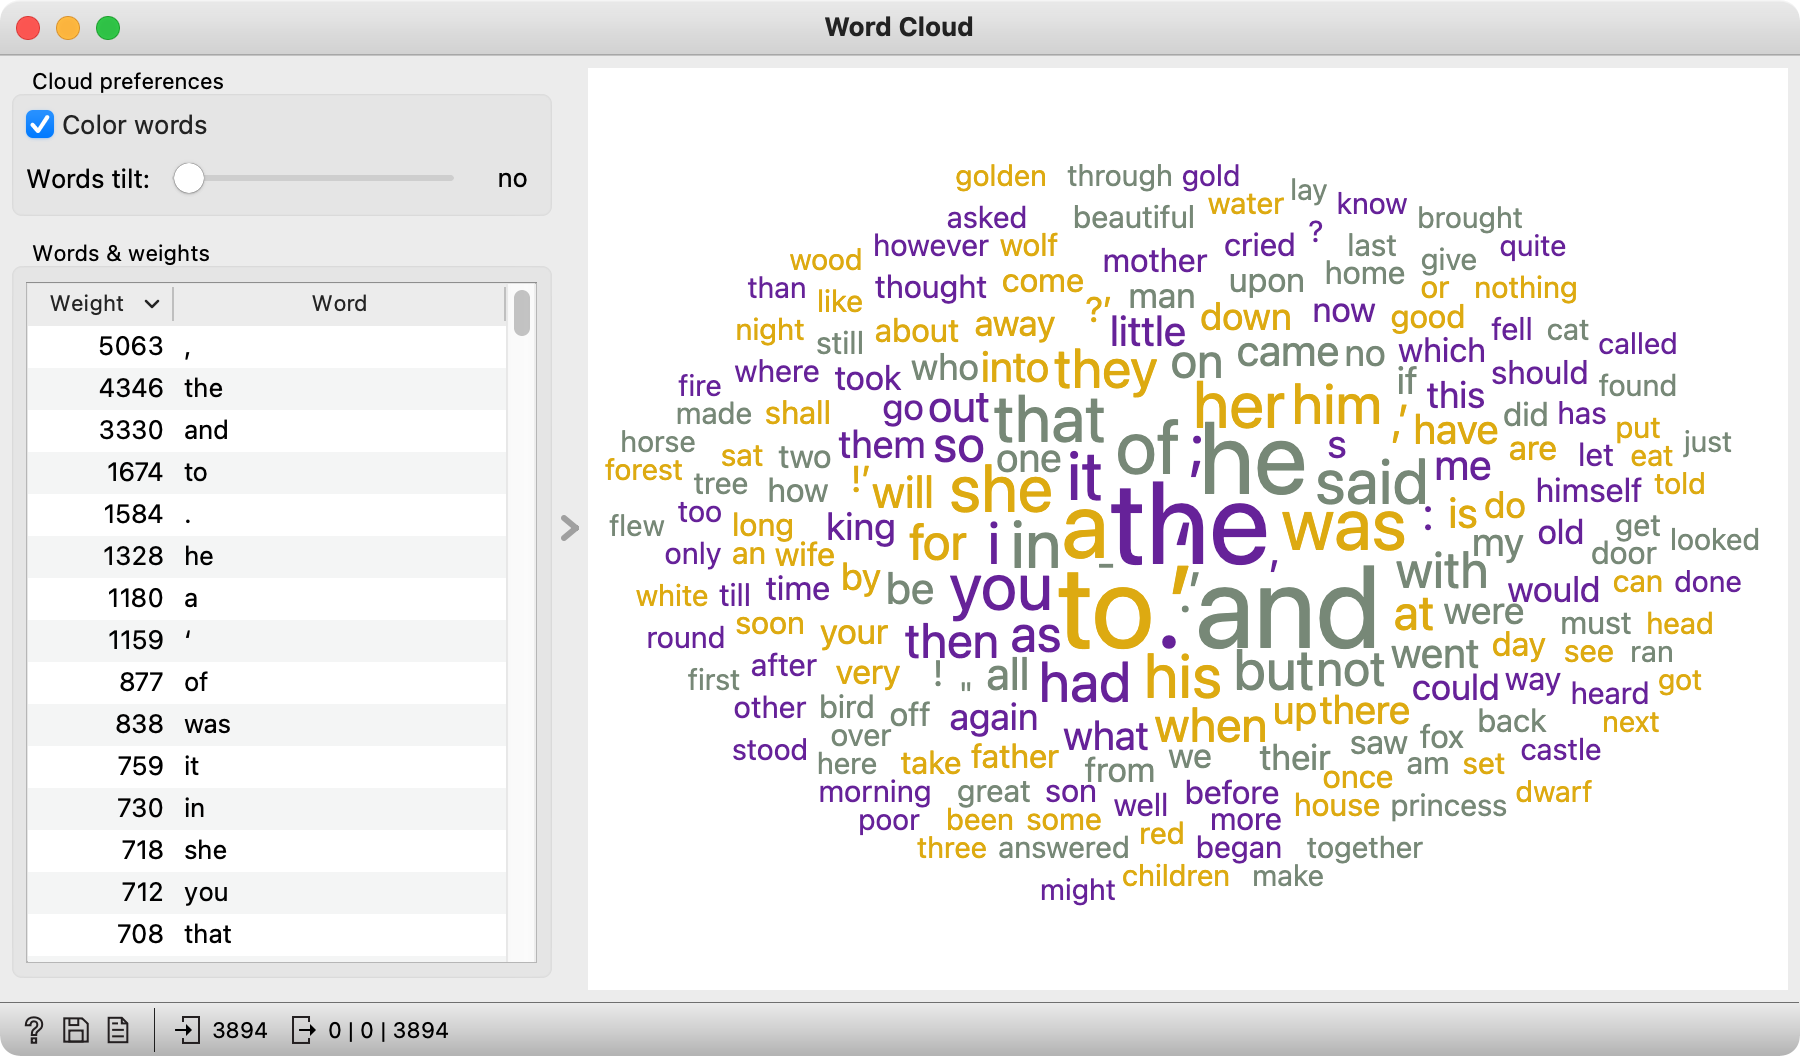
\includegraphics[width=\linewidth]{word-cloud.png}%
  \caption{$\;$}
\end{figure}
\vspace{-0.3cm}

But the word cloud we are looking at is a mess! We got a bunch of semantic junk in our visualization. Is there a way to clean this up?

Of course. One of the most important tasks in text mining is a correct preprocessing. We can achieve this with the \widget{Preprocess Text} widget.

\vspace{-0.2cm}
\begin{figure}[h]
  \centering
  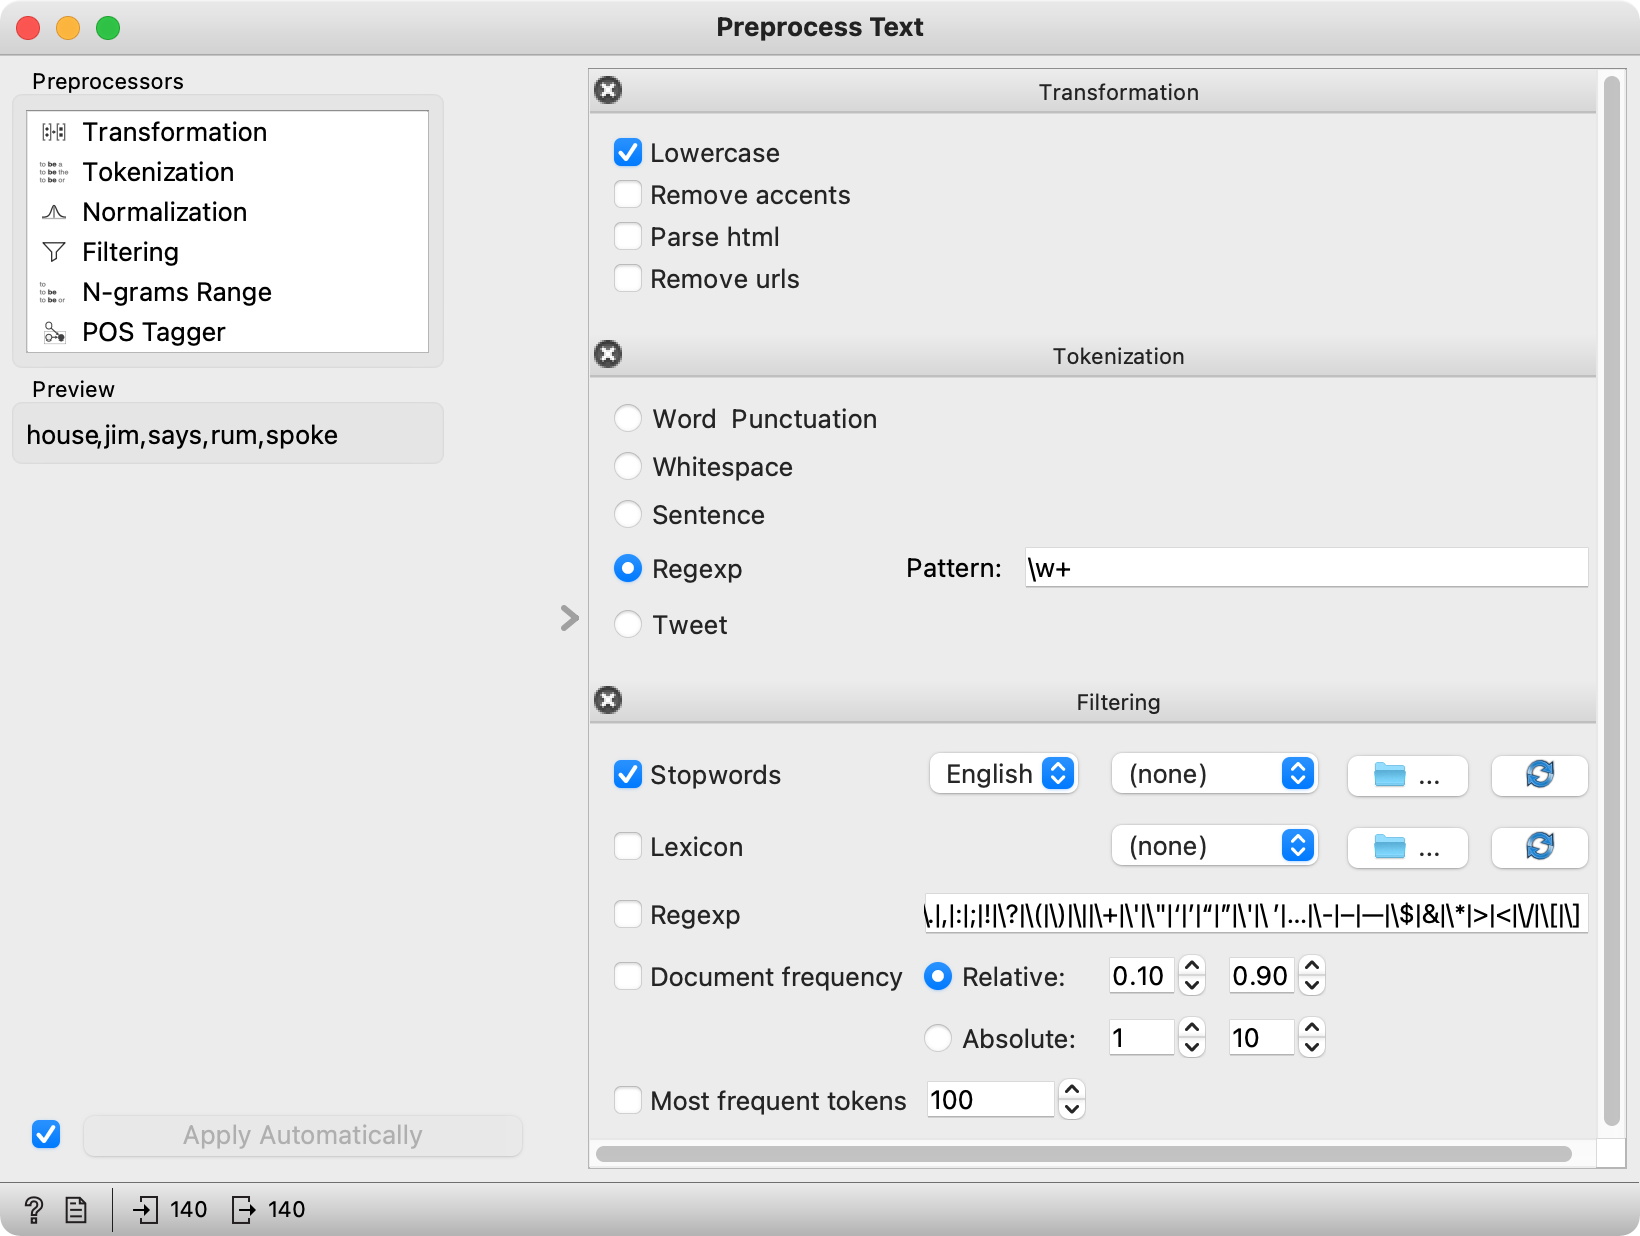
\includegraphics[width=\linewidth]{preprocess-text.png}%
  \caption{$\;$}
\end{figure}
\vspace{-0.3cm}

Preprocessing is executed sequentially. We start by lowercasing the text. This means words will be treated the same regardless of whether they appear at the beginning or middle of the sentence. However, words such as "apple" (a fruit) and "Apple" (a company) will also be treated the same, which is not always desirable.

\begin{wrapfigure}{o}{0.9\textwidth}
    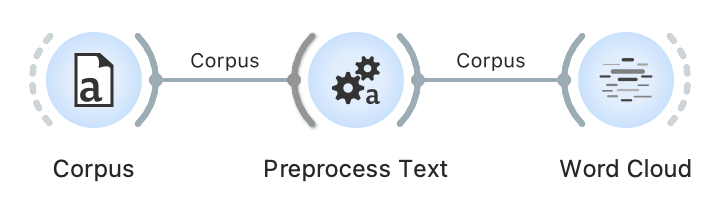
\includegraphics[scale=0.7]{workflow.png}
    \caption{$\;$}
  \end{wrapfigure}

Next, the text is split into \emph{tokens}, which are the core units of analysis. They are usually words, but they can also be sentences, bigrams, and so on. The default option, \emph{Regexp} keeps only words, omitting the punctuation.

We also removed redundant words. As we saw in the word cloud above, the most frequent words in English texts are "the", "and", "of", and so on. While these words are important for syntax, they do not carry any meaning, so they are often omitted from the analysis.

\marginnote{We see the results of our preprocessing in the Word Cloud. Two of the most frequent words are "would" and "could". If we decide these two words are not important for our analysis, it would be good to omit them. We can do this with custom filtering. filtered out some stopwords. But perhaps filtering out generic stopwords is not enough for our analysis.}

To sum up, we transformed all words to lowercase, treated each word as a token (and omit punctuation), and removed the stopwords (such as "in", "and", and "the"). This preprocessing outputs the following tokens:

"This is a sample sentence." $\rightarrow$ "sample", "sentence"

\vspace{-0.2cm}
\begin{figure}[h]
  \centering
  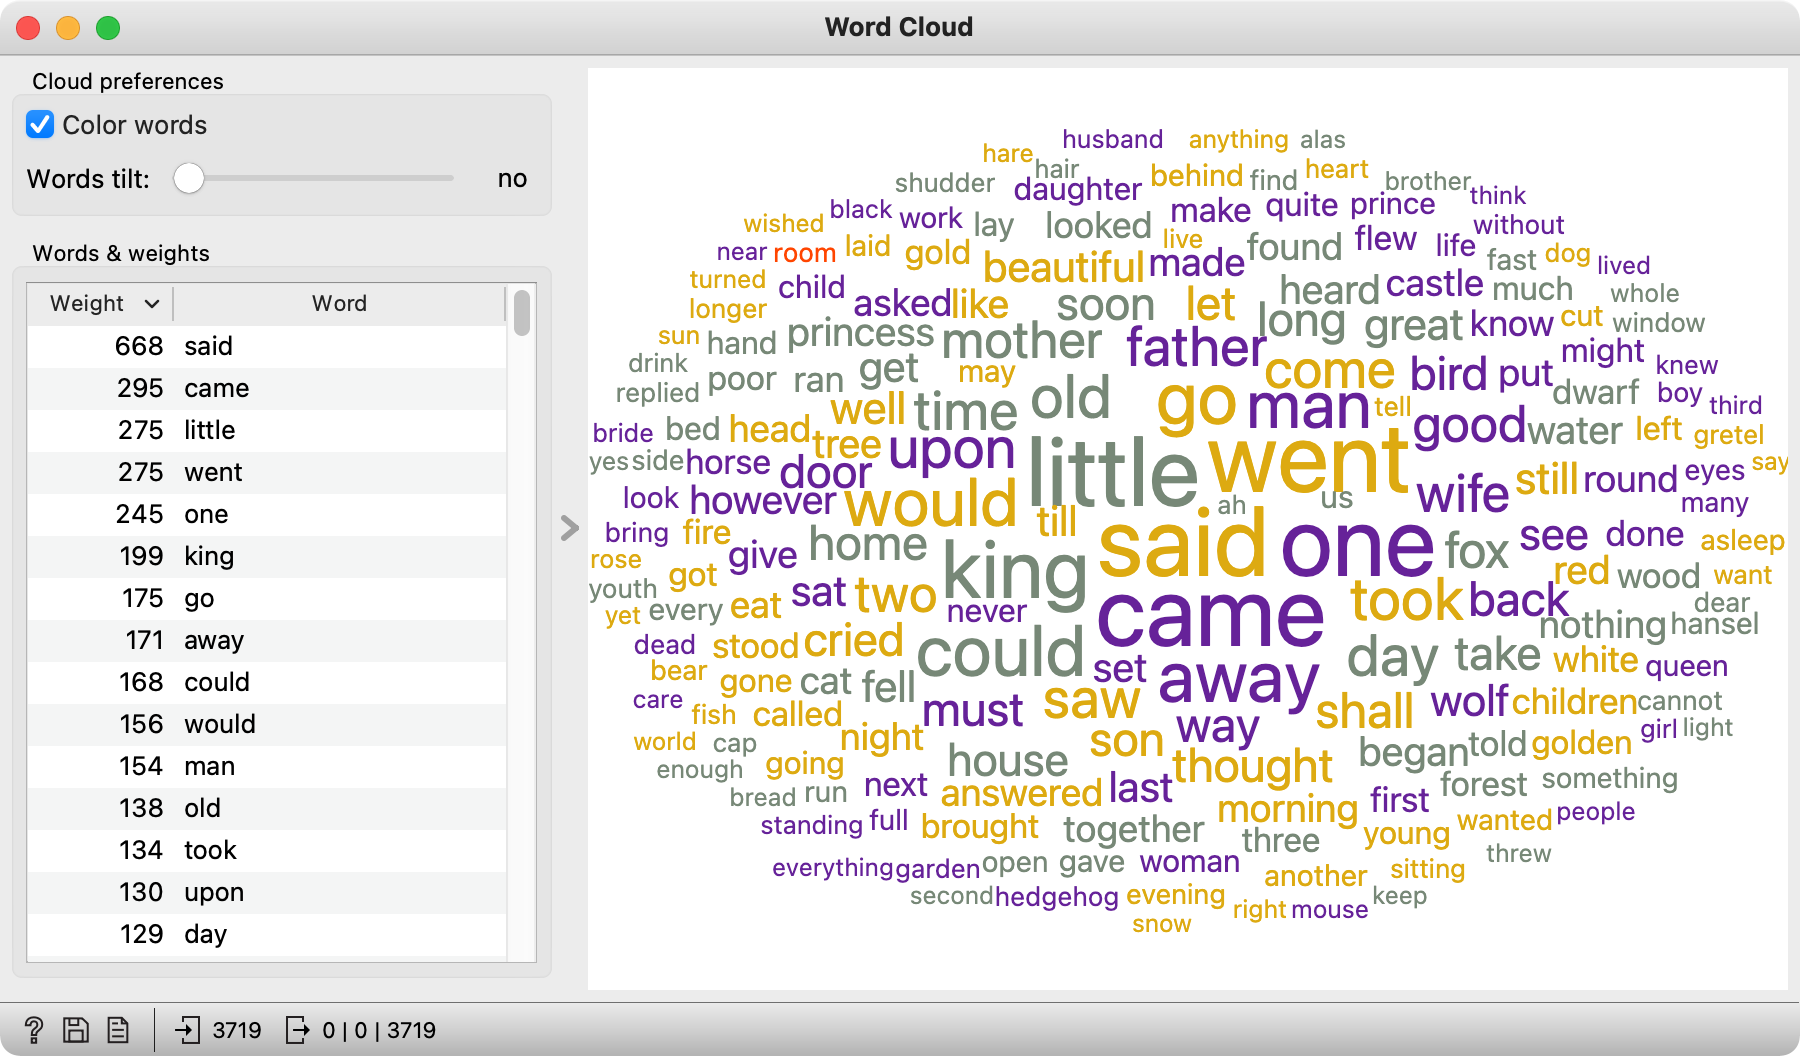
\includegraphics[width=\linewidth]{preprocessed-word-cloud.png}%
  \caption{$\;$}
\end{figure}
\vspace{-0.3cm}

We can always \marginnote{A good plain text editor is Sublime, but you can easily work with Notepad++.} load our own custom stopword list. Open a plain text editor and create a custom list of stopwords. Write each new word on its own line and save the file.

Load the list of custom stopwords in the right-hand dropdown of the Filtering section.

\begin{wrapfigure}{o}{0.5\textwidth}
  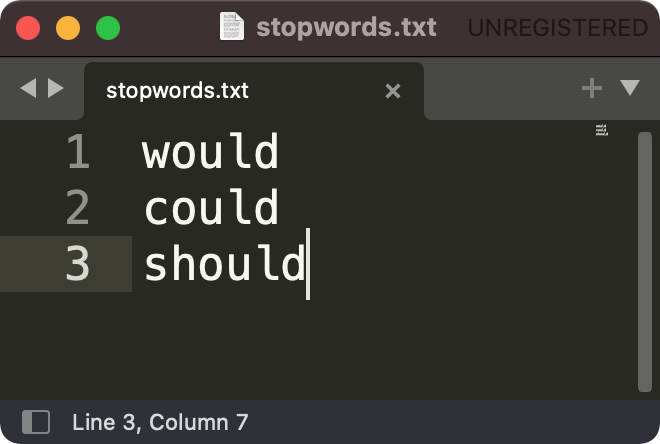
\includegraphics[scale=0.4]{editor.png}
  \caption{$\;$}
\end{wrapfigure}

Another preprocessing technique is to filter out words that are too rare and too frequent. Rare words are normally found in only a few documents and frequent words are likely stopwords or very general words. To retain only those words that truly represent the corpus and may distinguish between corpus documents, we use Document frequency filter with Relative frequencies. If we set the values to 0.1 and 0.9, we will retain only those words that appear in more than 10\% of the documents and in fewer than 90\%.

\newpage

\vspace{-0.2cm}
\begin{figure}[h]
  \centering
  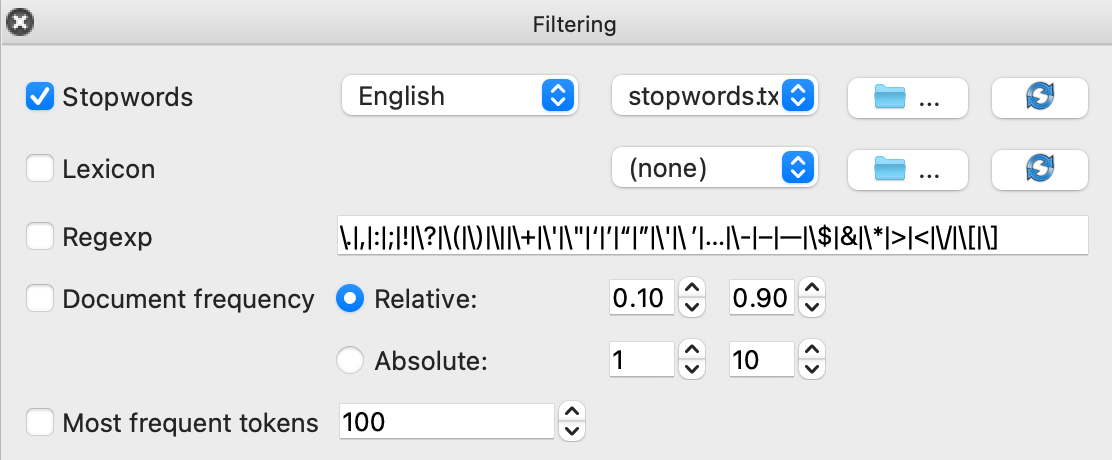
\includegraphics[width=\linewidth]{filtering.png}%
  \caption{$\;$}
\end{figure}
\vspace{-0.1cm}

Preprocessing is really the key to a successful text analysis. We have only mentioned a few techniques, but you can experiment on your own with the following ones:
\begin{enumerate}
\item normalization transforms all words into lemmas or stems (for example \emph{sons} to \emph{son})
\item n-grams are tokens of larger size, bigrams (a pair of consecutive words) and trigrams (word triplets)
\item POS tagging tags each token with a corresponding part-of-speech tag (\emph{sons} $\rightarrow$ noun, plural, tag = NNS)
\end{enumerate}

\vspace{-0.2cm}
\begin{figure*}[h]
  \centering
  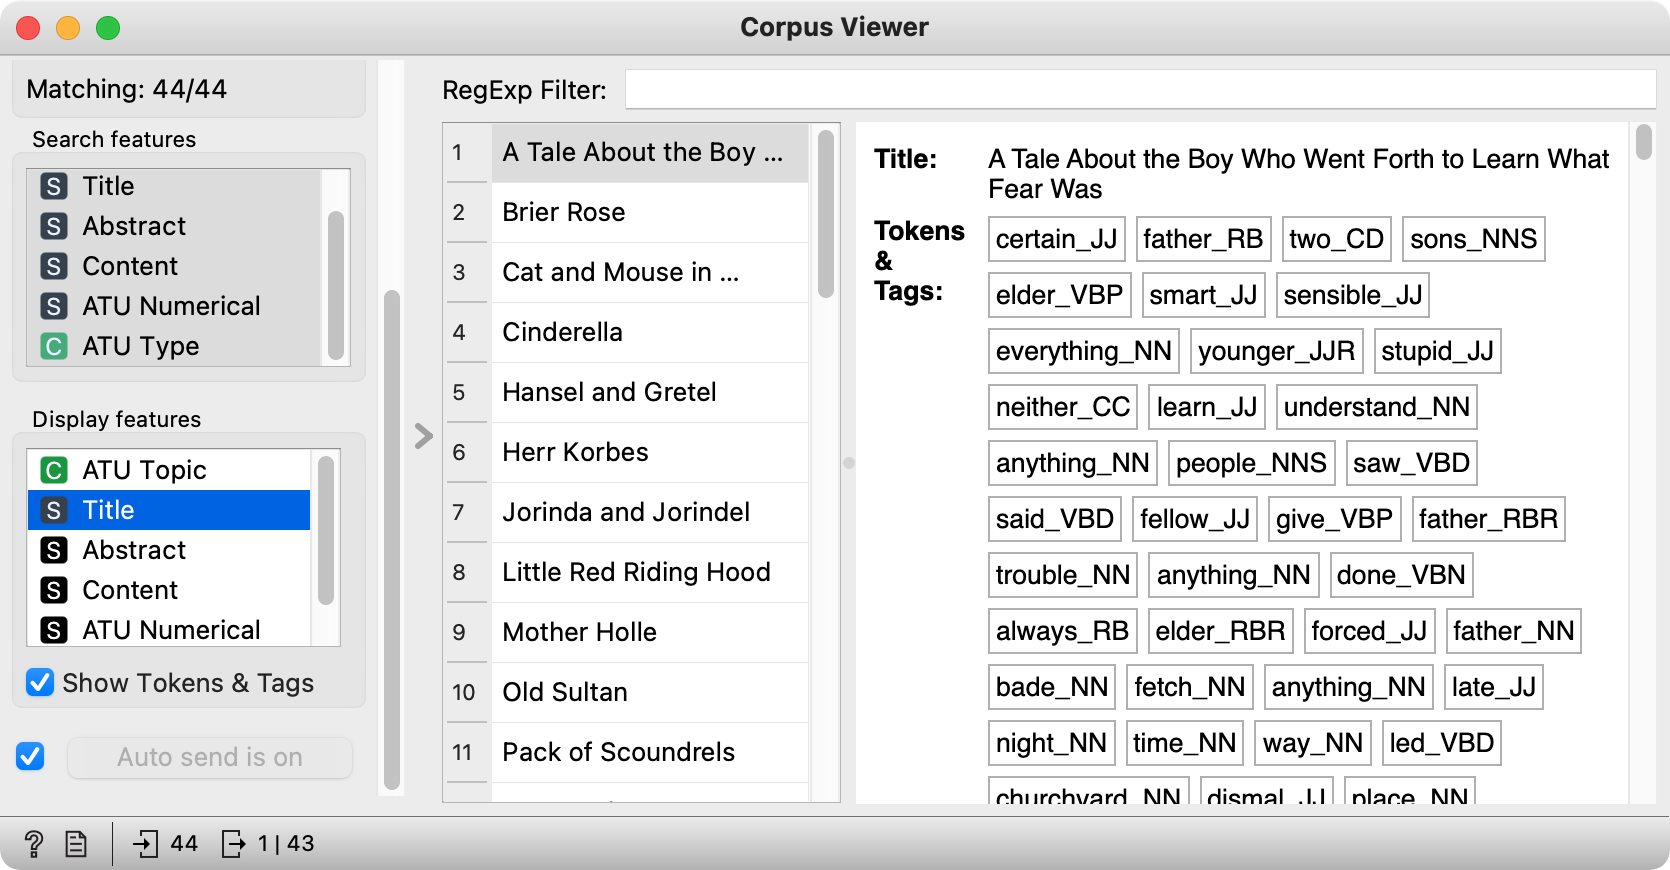
\includegraphics[width=\linewidth]{corpus-viewer.png}%
  \caption{$\;$}
\end{figure*}
\vspace{-0.3cm}
